\chapter{Design and development of the GNBot odor-sensing robotic platform}
\label{chap:design}
\vspace{-1cm}


For the robot design, existing open-source projects were used as a base. The preferred designs had most mechanical parts intended to be manufactured with a low-cost 3D printer. These are called \emph{printbots} \cite{GonzalezValero11miniskybot, ValeroGonzalez12creativity, ValeroGonzalezOOML12}, and one example is the MiniSkybot\footnote{\url{http://www.iearobotics.com/wiki/index.php?title=Miniskybot\_2}}. Printbots provide an accelerated design path not only for creating basic educational tools \cite{Garcia-Saura2012} but also for making robots that can be used for research, such as the platform presented in this work.
With this technique it is possible to easily reuse, develop and incorporate the most useful parts of previous designs in order to fulfill the requirements of a robot needed for a given task.

Regarding swarm robotics, printbots have been preferred over other solutions for both the reduced manufacture cost and, most importantly, for the high adaptability of the designs to the search problems. For instance, the use of 3D printed structures opens the possibility of easily testing the performance of various spatial distributions of the odor sensors in the robot, by manufacturing custom parts that can accommodate the different configurations.




The proposed robot design (shown in Fig. \ref{fig:design/GNBot_iterations}) is a derivative of the ArduSkybot\footnote{\url{https://github.com/carlosgs/ArduSkybot}}, an educational printbot based on the Arduino\footnote{\url{http://arduino.cc}} UNO electronic board, and it also incorporates work from the Vector-9000\footnote{\url{https://github.com/carlosgs/carlosgs-designs/tree/master/Vector-9000-a-fast-line-follower-robot}} competition robot. 
From these projects, integration was made in respect to hardware (mechanical parts and electronic boards) and software (robot firmware and a basic communication strategy) aspects.
On the hardware side, the ArduSkybot design was modified to incorporate the Arduino MEGA board to allow the addition of more sensors.

%\vspace{1cm}

\begin{figure}[h!]
\centerline{\mbox{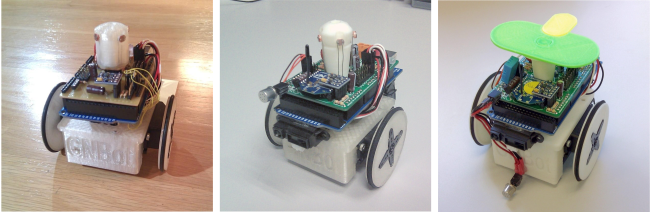
\includegraphics[width=16cm]{images/design/GNBot_iterations.eps}}}
\captionFigure{The three GNBot versions that were developed}
{fig:design/GNBot_iterations}{
From left to right: GNBot version alpha, v0.1 and v1.0 (the current version).
The two earlier designs had a light sensor array placed on the top (intended for light landmark identification as shown in Appendix \ref{Appendix:lightLandmarks}), while the latest version has a two-color marker (intended for the automated visual position tracking in Section \ref{sect:visionBasedLocalization}). %Both subjects are explained in further sections.
}\end{figure}

\vspace{-1cm}



\lsection{Open-source electronics}
\label{sect:openSourceElectronics}


The Printshield board -designed for the ArduSkybot- was the base to design the GNBoard (see Fig. \ref{fig:design/GNBoard_prototypeAndFinal}), which provides a compact solution that contains most sensors and allows an easier interconnection. The GNBot also incorporated a light sensor array developed originally for the Vector-9000, and that project also provided the software base with a framework to interface with the computer in a fault-tolerant manner. All of the PCB designs (schematics and circuit layout) were designed using the \emph{KiCad EDA Software Suite}\footnote{\url{http://www.kicad-pcb.org/}}, an open-source tool.




\begin{figure}[h!]
\centerline{\mbox{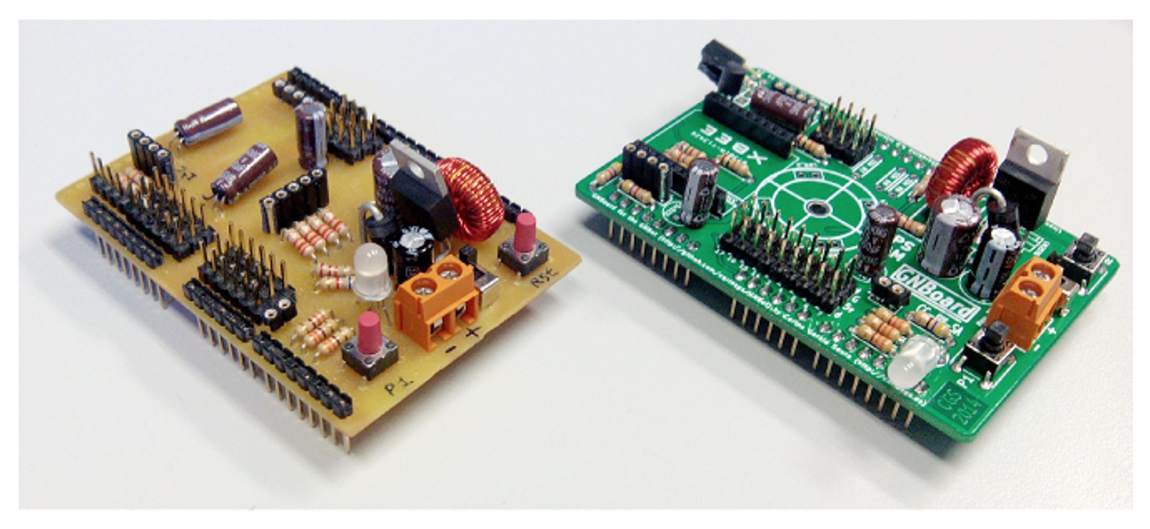
\includegraphics[width=15cm]{images/design/GNBoard_prototypeAndFinal.eps}}}
\captionFigure{The two versions of the GNBoard developed for this project}
{fig:design/GNBoard_prototypeAndFinal}{
Prototype design (left) and version 1.0 (right).
The boards are designed to plug into an \emph{Arduino MEGA}.
Schematics and layout can be found in Appendix \ref{Appendix:circuits}.
}\end{figure}






The motion of the robot is achieved using two continuous rotation servomotors (\emph{SM-S4303R}) as the main actuators. Servomotors provide a compact and low-cost solution to achieve the digital speed control needed, and they are frequently used in bio-inspired robot designs \cite{zamorano2011control,Herrero11,Urziceanu11,MeyerSproewitz06}.
%\cite{zamorano2011control} % Control locomotor multidireccional de un robot modular mediante circuitos generadores centrales de patrones bioinspirados
%\cite{Herrero11} % Bio-inspired design strategies for central pattern generator control in modular robotics
%\cite{Urziceanu11} % Central pattern generator control of a differential wheeled robot
%\cite{MeyerSproewitz06} % Passive compliance for an ({RC}) servo-controlled bouncing robot
The main downside of this kind of actuator is the high current demand -particularly during transient motions- which requires the use of an adequate power supply. For the GNBoard the design decision was to use a switching power supply (shown in Fig. \ref{fig:design/GNBoard_PSU}) rather than a linear regulator, provided the much higher efficiency.
\begin{figure}[h!]
\centerline{\mbox{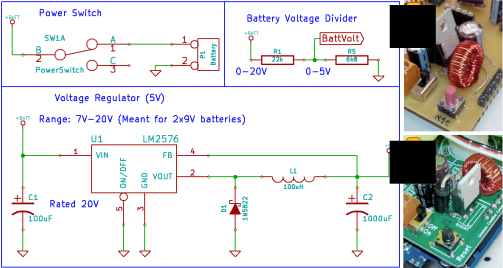
\includegraphics[width=12cm]{images/design/GNBoard_PSU.eps}}}
\captionFigure{Power supply schematic and actual assembly}
{fig:design/GNBoard_PSU}{
\emph{A)} and \emph{B)} respectively show the power supplies in GNBoard v0.1 and v1.0 (final version).
The power supply of the GNBoard uses an \emph{LM2576-5} switching regulator that is capable of delivering up to 3A, which is more than sufficient to cover the energy demand of the entire robot.
}\end{figure}
Switching power regulators also have a broad input voltage range, allowing to make better use of the full capacity of the batteries since they can be connected in series without negative effect in the performance.

The other incorporated element was a battery voltage monitor, which has been designed to be used for resource-wise decision making in search strategies. The implementation of this sensing capability was done by placing a resistive voltage divider (also shown in Fig. \ref{fig:design/GNBoard_PSU}) that adapts battery voltage to the $[0,5]V$ range that can be measured with the Arduino board.


The selection of sensory input was oriented towards the odor source localization task, and thus an electronic nose was made part of the robot (see Fig. \ref{fig:design/artificialNose_polarization}).

\begin{figure}[h!]
\centerline{\mbox{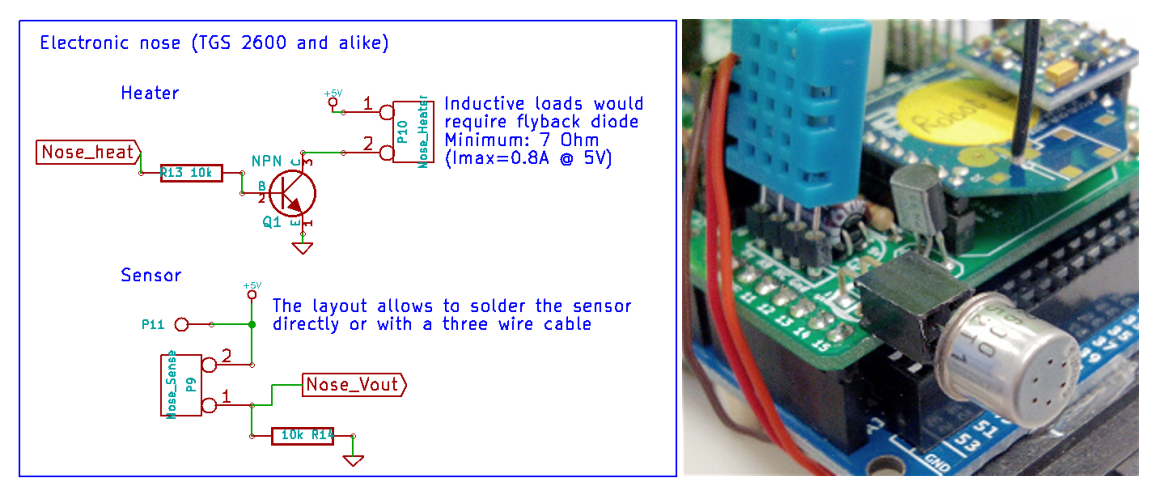
\includegraphics[width=14cm]{images/design/artificialNose_polarization.eps}}}
\captionFigure{Polarization scheme for the artificial nose sensor and detail picture of the assembly}
{fig:design/artificialNose_polarization}{
The mounted sensor is the \emph{TGS-2600} gas detector from \url{http://www.figarosensor.com/}, but any kind of sensor with a similar polarization scheme (as shown in the left panel) could be used.
}\end{figure}

The odor sensor works with a heater element whose temperature can be controlled electronically by a power transistor placed for this purpose on the GNBoard.
Odor sensor temperature control allows the usage of different modulation strategies to enhance sensor performance and to allow adaptation to the intensity of odor sources \cite{YanezToledano12}. 
Robots also incorporate an infra-red analog rangefinder (ref: \emph{Sharp GP2Y0A21}) to avoid collision with obstacles and other robots within the search environment, as well as a light sensor array intended to be used to identify light landmarks.
A temperature and humidity sensor (ref: \emph{Aosong DHT11}) is also present in the GNBoard.
Finally, an electronic compass (ref: \emph{Honeywell HMC5883L}) provides the orientation knowledge.
This way, each robot and the swarm can have a basic multimodal perception of their status and location in the search area.

Overall the GNBoard designed for this project allows the incorporation of multiple sensors and facilitates software-hardware integration, as it is an essential requirement for the efficient implementation of odor search tasks that have uncertainty. Next section will cover the selection of the communication system.


\vspace{-0.5cm}

\lsection{Communication with the robots}

In the case of collaborative swarm robots, one of the key design decisions that needs to be made is the selection of a proper communication method. Not only there is a trade-off between the \emph{working range, maximum information throughput and cost}, but there are some other facts that must also be taken into account:
\begin{packed_itemize}
\item \emph{Working environment:} Radio-Frequency (RF) communications generally provide a robust system for most applications, but sometimes other solutions can provide a better balance between performance and cost. For instance, for underwater applications RF signal attenuation may become an issue, and the use of sound waves, light pulses, or even tethering with a cable become reasonable options.
\item \emph{Power requirements, adaptivity and remote-end sensing:} Since mobile robots have very limited energy resources, an efficient system should be generally preferred in order to maximize the operation time. In the same line, some interfaces provide a way to switch among different power schemes in real time, as well as having the capability to measure the signal intensity received from the other end. These should be preferred since the adaptivity in communications is key towards an optimal usage of energy resources.
\item \emph{Networking capability:} Not all communication systems offer the possibility to address data to different end nodes, and this is a must to allow scaling up the size of the swarm. This factor is crucial towards the efficient implementation of inter-robot communication.
\end{packed_itemize}

ZigBee\footnote{\url{http://www.digi.com/technology/rf-articles/wireless-zigbee}} (\emph{IEEE 802.15.4}) has been chosen from all of the available integrated solutions, since it is a highly configurable platform that is compatible with most of the points detailed above (see Table \ref{tab:design/xbee_wifi_bt_comparison} for a technical comparison). It provides an excellent networking layer, and since it is designed for low power applications, ZigBee has the possibility of adapting RF energy usage in real time.


\begin{table}[h!]
\centerline{\mbox{\includegraphics[width=12.5cm]{images/design/xbee_wifi_bt_comparison.png}}}
\captionTable{Comparison of the ZigBee, GPRS/GSM, Wi-Fi and Bluetooth wireless communication protocols}
{tab:design/xbee_wifi_bt_comparison}{
Source: ZigBee Alliance
}\end{table}


The main downsides of the ZigBee solution are the maximum throughput rates and the timing constrains, which must be taken into account when considering the use of more complex sensory input such as real time video streams.

Incorporation of the ZigBee modules into the GNBoard needed some special considerations (see Fig. \ref{fig:design/GNBoard_ZigBee}), as the selected modules work on 3.3V signals while the Arduino and GNBoard run on 5V.

\begin{figure}[h!]
\centerline{\mbox{\includegraphics[width=14cm]{images/design/GNBoard_ZigBee.eps}}}
\captionFigure{ZigBee connection schematic and its actual place in the GNBoard}
{fig:design/GNBoard_ZigBee}{
The selected ZigBee-compatible module is the \emph{XBee S2 (XB24-BWIT-004)}.
A 3.3V power line was reutilized from the regulator already present in the Arduino MEGA board. Adaptation of the TTL signal levels for the $Arduino \rightarrow ZigBee$ path was done using a resistive voltage divider. The $ZigBee \rightarrow Arduino$ path, on the other hand, did not require adaptation of the voltage level, since 3.3V TTL is correctly interpreted by the Atmel processor present in the Arduino board.
A decoupling capacitor was added to the 3.3V power line, and both of the transmission lines are terminated with resistors in order to maximize signal integrity.
}\end{figure}




Communication with the robots through these modules is asynchronous with a best-effort policy for packet forwarding, and thus real time event handling is critical. Data links must be fault tolerant, which can be achieved by using redundancy to ensure that messages are received and processed correctly by each node, and soft-state should be preferred to avoid deadlocks and allow fast recovery.
Reliability in communications is a key element to implement the virtualized network topology explained in next section.


\subsection{The ZigBee-based abstraction layer}

Odor search algorithms may rely on very different network topologies to maximize the chances of successful search and minimize time or energy consumption while, at the same time, dealing with context-specific communication range restrictions. In particular, the spatial scale of the search problem and the actual detection range of the odor sources are important factors to design the network topology, which could be changed for instance according to the energy level information.
As shown in Figure \ref{fig:design/topology}, a base tree topology makes it possible to emulate and test many different architectures.



\begin{figure}[h!]
\centerline{\mbox{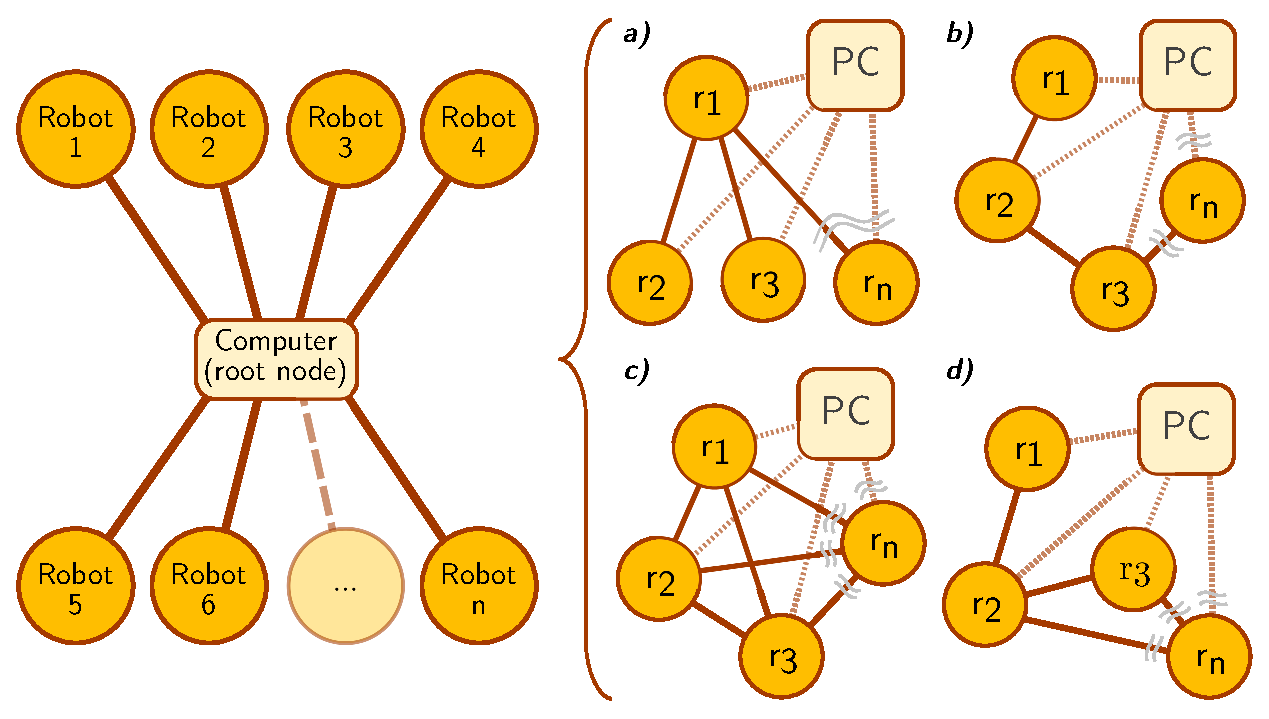
\includegraphics[width=15cm]{images/design/topology.eps}}}
\captionFigure{Possible virtualizations of the network topology}
{fig:design/topology}{
The star architecture shown on the left serves as the base to emulate a wide range of topologies. While underlying communications are centralized, the implemented algorithms can have very different requirements. As all information flows through the central computer, virtualized connectivities between robots can be defined in order to achieve various architectures such as \emph{a) tree/star}, \emph{b) line}, \emph{c) fully interconnected}, or \emph{d) mesh}, among others. The emulation of many other characteristics of physical links (\emph{variable delays, jitter, data corruption, packet loss...}) could be used to test the resilience of the implemented search algorithms in a controlled manner.
}\end{figure}


The approach used is to abstract all the calculations to a root computer, effectively using each robot as a peripheral.
A centralized infrastructure is used to command each autonomous robot independently, but a convenient layer of abstraction will also allow testing algorithms that are decentralized (see panels \emph{a-d} in Fig. \ref{fig:design/topology}). Main advantages of this approach are:
%\begin{packed_itemize}
\begin{itemize}
\item First, it is able to reduce costs since robots are kept simple, with reduced computational ability. For a fixed funding, cutting down the cost of each robot makes it possible to create more of them and thus have a bigger swarm.
\item Second, as all data flows through the root node, it can be logged and analyzed in order to evaluate the performance of each algorithm and allows easier debugging. Having all information in one place is particularly convenient when testing distributed algorithms.
\item Third, it provides a layer of abstraction. The code that specifies the behavior of each robot runs on the central computer, and thus a high-level programming language can be used (Python\footnote{\url{http://www.python.org/}} was selected for this project). This way it is possible to focus on developing the algorithms rather than dealing with the limitations of memory and power of the micro-controller on board each robot.
\item Finally, it is important to emphasize that the centralized architecture supports a large dynamic range of complexity of the algorithms, that can be kept simple (i.e. chaotic search~\cite{KongcunM09}) or complex (i.e. particle filtering~\cite{Marques2006}).
\end{itemize}
%\end{packed_itemize}

The emulated topologies could be dynamically reconfigured in real time to adapt to the search requirements (i.e. groups of robots may establish separate sub-networks when getting far from others to do local search, and later share the search results with the rest of the group).
The chosen ZigBee communication protocol natively supports the deployment of such architectures in the real world, which makes it very convenient towards the actual implementation of the virtually-optimized topologies.











\lsection{Real time robot position measurement}
\label{sect:realTimePositionMeasurement}

Knowledge of the position that each robot has in the area of the experiment is not only needed as input for some search strategies, but also for the evaluation of the performance of search algorithms in general. The trajectories undertaken by each robot can be useful information that allows the measurement of redundancy, interaction and efficiency during the performance of an odor localization task.

For this project, a new multimodal approach for robot localization was developed and evaluated. The idea was to use purposely-placed light sources as landmarks that allow each robot the identification of their relative positions within the search area. Unfortunately, the electronic compass sensor that provided the orientation measurements needed did not perform as expected (due to magnetic field distortion indoors) and the method had to be discarded for its noisy position results. All the information regarding this technique can be found in Appendix \ref{Appendix:lightLandmarks}.


\subsection{Vision-based robot localization}
\label{sect:visionBasedLocalization}

Among the other robot localization approaches studied, the most convenient method was the use of computer vision algorithms in combination with visual markers on board each robot.
This technique required the use of an external camera observing the space where robots move, as well as color markers placed in the robots.
The developed visual markers (in Fig. \ref{fig:design/GNBot_opencv_markers}) were designed to be 3D-printed, as are the rest of the GNBot parts.
These markers have two distinguished colors in order to achieve the measurement of both XY position and rotation of the robots.
Rotation feedback is also necessary since the electronic compass measurements had proved to be quite noisy for indoor spaces (see Appendix \ref{Appendix:lightLandmarks}).





%\subsubsection{Design of the visual position markers}

\begin{figure}[h!]
\centerline{\mbox{\includegraphics[width=12cm]{images/design/GNBot_opencv_markers.png}}}
\captionFigure{GNBot general purpose attachment piece and 3D-printed visual markers}
{fig:design/GNBot_opencv_markers}{
First and final versions of the markers used for computer-vision robot localization are shown in the left and right respectively. The part in the center is the attachment piece that allows to mount these markers and any other custom parts into the GNBot.
}\end{figure}







For measuring 2D positions, at first glance the best place for the external camera would be the ceiling right over the monitored area, in order to minimize distortion.
That way it would be possible to linearly map the observed robot position in the camera video with its actual location in the real world.
But as manually obtaining an adequate camera alignment is laborious and error-prone, another solution can be to calibrate the camera position using image processing software. Perspective correction
(see Fig. \ref{fig:design/perspective_correction})
simplifies this process: the user only needs to specify the position within the captured video of four reference points whose real location and dimensions are known.
\begin{figure}[h!]
\centerline{\mbox{\includegraphics[width=11cm]{images/design/perspective_correction.png}}}
\captionFigure{Example of the video perspective correction}
{fig:design/perspective_correction}{
The original video stream is shown on the left, and the result of the perspective correction is shown on the right. The perspective has to be corrected in order to account for the visual distortion of the observed targets. This way, the X-Y position of each robot becomes linearly-proportional to the pixel positions in the video stream and can be directly mapped.
}
\end{figure}
The perspective correction technique is commonly used in many fields such as the aerospace industry for satellite surveillance or animal tracking for neuroethological research.

OpenCV\footnote{\url{http://www.opencv.org/}} was used for implementing the marker tracking software, as it is a convenient library that provides an efficient bundle of all the necessary image processing functions.
The full tracking process is explained in Figures \ref{fig:design/opencv_tracking_steps} and \ref{fig:design/opencv_tracking_steps_angle}.



\begin{figure}[h!]
\centerline{\mbox{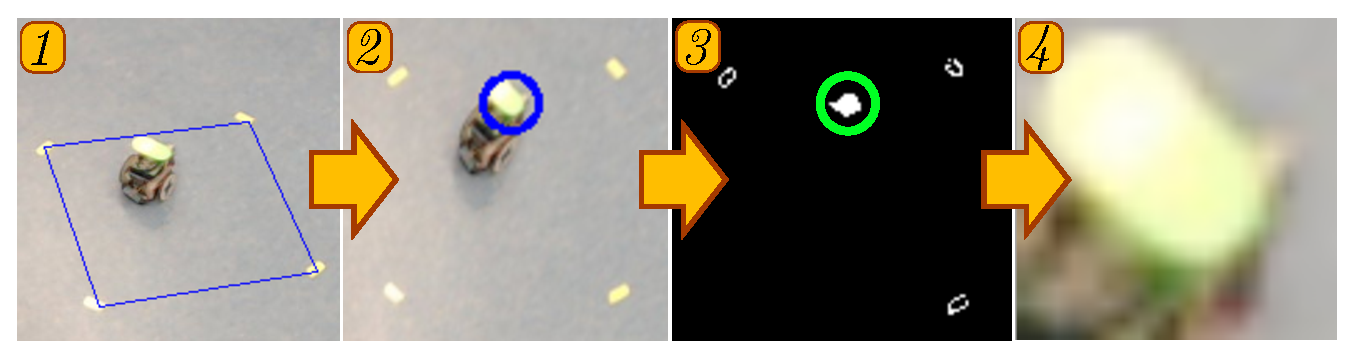
\includegraphics[width=15cm]{images/design/opencv_tracking_steps.eps}}}
\captionFigure{Steps of the marker position detection algorithm}
{fig:design/opencv_tracking_steps}{
In a first step, the user manually specifies the reference points in the original video stream \emph{(1)} by using the mouse. The rest of the process is automated, with the creation of a corrected perspective image \emph{(2)}, the application of a threshold that focuses on the marker color \emph{(3)}, and the detection of the largest spot, which will finally output the coordinates of the robot. Afterwards, the \emph{region of interest} is segmented \emph{(4)} for the next step of the algorithm: robot orientation measurement (see Fig. \ref{fig:design/opencv_tracking_steps_angle}).
}\end{figure}




\begin{figure}[h!]
\centerline{\mbox{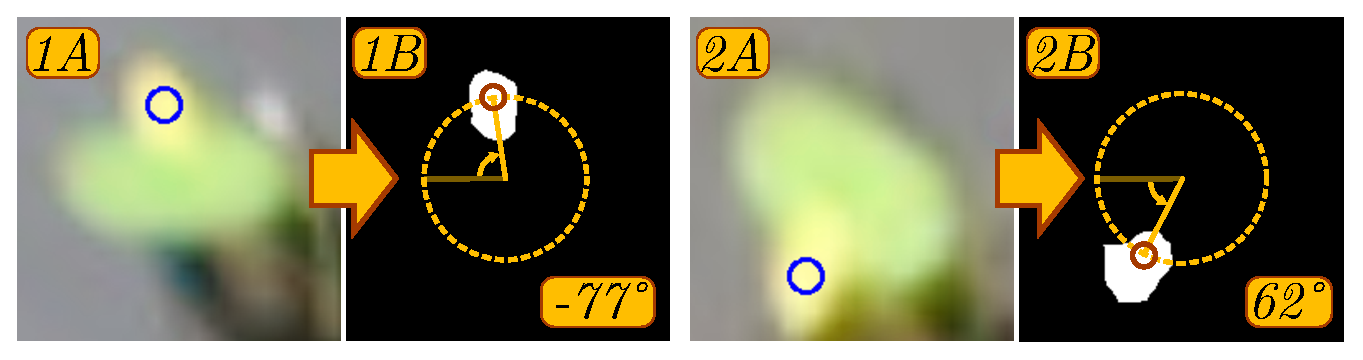
\includegraphics[width=15cm]{images/design/opencv_tracking_steps_angle.eps}}}
\captionFigure{Marker orientation detection algorithm}
{fig:design/opencv_tracking_steps_angle}{
\emph{1A} and \emph{2A} show the segmented ``region of interest'' from the previous part of the tracking algorithm (see Fig. \ref{fig:design/opencv_tracking_steps}), displaying the corrected-perspective marker in the middle. As the largest color of the marker (green) is centered, it is then possible to apply a threshold \emph{(2A},\emph{2B)} that focuses on the sub-marker (yellow) to obtain its position. Finally, the robot rotation angle is calculated according to the relative position of the sub-marker with respect to the center.
}\end{figure}


The software was fully implemented in Python for this project, using only standardized OpenCV functions (\texttt{cv2.getPerspectiveTransform}, \texttt{cv2.warpPerspective}, \texttt{cv2.cvtColor}, \texttt{cv2.inRange}, and \texttt{cv2.findContours}).
Also, the developed system is open-source and can be easily re-purposed for other video tracking tasks.



\vspace{-0.5cm}
\lsection{3D-printable hardware design}
\vspace{-0.2cm}
From the specification of the project, the GNBot design was oriented towards cost reduction and easy replication.
Fig. \ref{fig:design/GNBot_parts} shows all the components that are needed to assemble one robot, and the resulting GNBot is shown in Fig. \ref{fig:design/GNBot_views}.

\begin{figure}[h!]
\centerline{\mbox{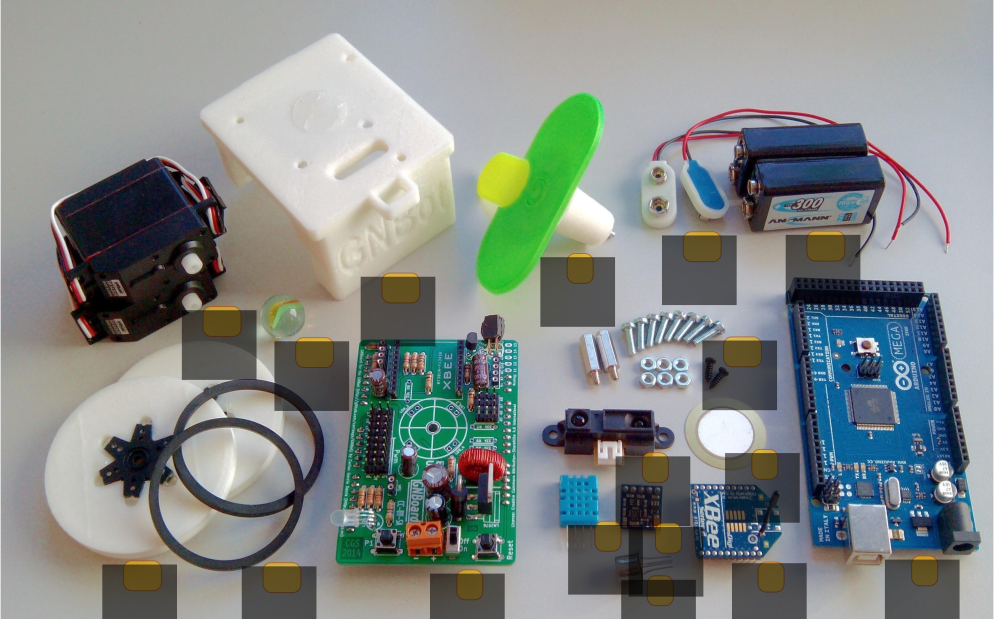
\includegraphics[width=16cm]{images/design/GNBot_parts.eps}}}
\captionFigure{Detail of the parts that form one GNBot v1.0}
{fig:design/GNBot_parts}{
Items shown in the picture:
\emph{1)} GNBoard electronics.
\emph{2)} Arduino MEGA board.
\emph{3)} TGS-2600 odor sensor.
\emph{4)} ZigBee-compatible RF module.
\emph{5)} Infra-red distance sensor.
\emph{6)} DHT11 temperature and humidity sensor.
\emph{7)} HMC5883L magnetometer sensor.
\emph{8)} Piezoelectric buzzer.
\emph{9)} Visual marker attachment.
\emph{10)} Two 9V battery connectors.
\emph{11)} Two 9V rechargeable batteries (300mAh).
\emph{12)} Two continuous-rotation servomotors.
\emph{13)} 3D-printed robot wheels.
\emph{14)} Rubber outer-wheel rings.
\emph{15)} 3D-printed GNBot chassis.
\emph{16)} Marble for the idler wheel.
}\end{figure}

%\vspace{-0.2cm}
The only custom items that are present in the design are the GNBoard electronics and the 3D-printed parts (robot chassis, wheels and battery holder), which can be manufactured at a low cost. All of the other components are standardized and widely available.
The assembly of each robot is a simple process that only requires the use of standard tools (a flathead screwdriver, cutting pliers, and a hot-melt glue gun).

\begin{figure}[h!]
\centerline{\mbox{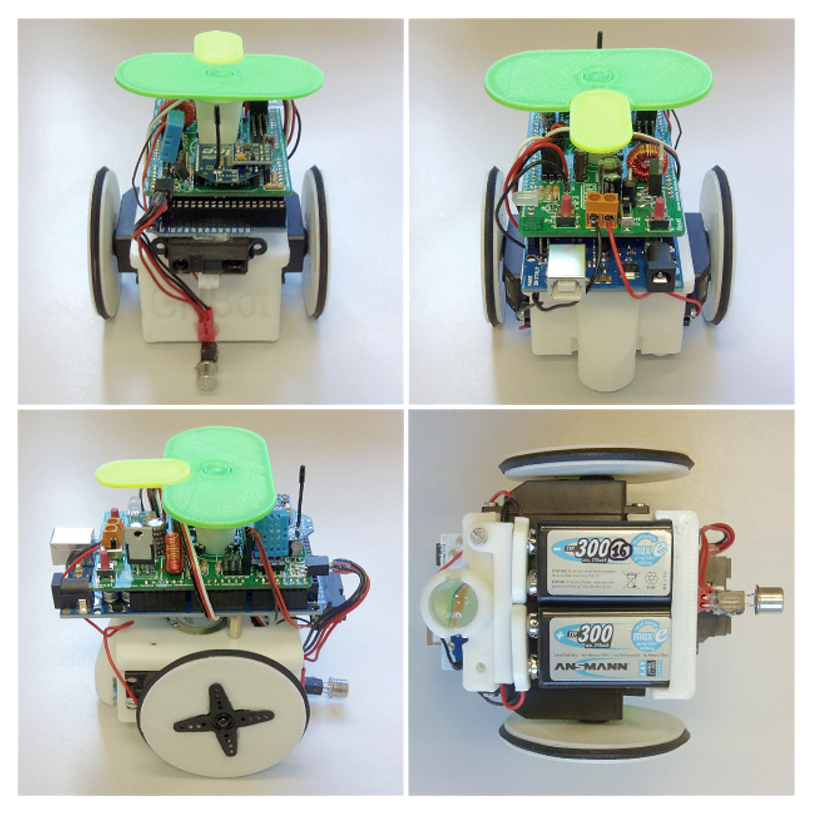
\includegraphics[width=13.5cm]{images/design/GNBot_views.eps}}}
\captionFigure{Assembled GNBot v1.0}
{fig:design/GNBot_views}{
Front, rear, side and perspective views. List of sensors present in the robot:
TGS-2600 odor sensor, IR rangefinder, LDR light sensor array, electronic compass module, temperature and humidity sensors.
Battery voltage is also monitored.
The base actuators are two servomotors and the wireless interface is based on a ZigBee-compatible module.
}\end{figure}




\newpage \thispagestyle{empty} % Página vacía

